\chapter{الخلية، وحدة الحياة}\label{ch:g6:cell-unit-of-life}

انتهى \cref{ch:g5:first-look-at-cells} بوعد: الغرف الصغيرة ليست
خاوية. وهذه السنة يخرج \omterm{def:g5:first-look-at-cells:microscope}{مجهر} المدرسة من جديد --- بشرائح أفضل
وأسئلة أحدّ. فماذا في \omterm{def:g5:first-look-at-cells:cell}{الخلية} بالضبط؟ وهل تختلف \omterm{def:g5:first-look-at-cells:cell}{الخلية} النباتية عن
الحيوانية؟ وهل \omterm{def:g5:first-look-at-cells:cell}{الخلية} \emph{جزء} من الحياة، أم يمكن أن تكون \omterm{def:g5:first-look-at-cells:cell}{خلية}
واحدة كائنًا حيًّا كاملًا؟ إن أصغر وحدة في \omterm{def:g1:living-or-not:living}{علم الأحياء} تستحق فصلًا
وافيًا.

\section{داخل الخلية}

\begin{definition}[أجزاء الخلية]\label{def:g6:cell-unit-of-life:parts}
إذا نُظر إليها كما ينبغي، أظهرت كل \omterm{def:g5:first-look-at-cells:cell}{خلية} العتاد الأساسي نفسه:
\begin{enumerate}
  \item \emph{الغشاء}\index{غشاء}، وهو غلاف \omterm{def:g5:first-look-at-cells:cell}{الخلية} الخارجي
        الرقيق، يمسكها ويضبط ما يدخل وما يخرج؛
  \item و\emph{السيتوبلازم}\index{سيتوبلازم}، وهو الحشوة الهلامية
        التي يجري فيها عمل \omterm{def:g5:first-look-at-cells:cell}{الخلية}؛
  \item و\emph{النواة}\index{نواة}
        (وهي البقعة الداكنة في
        \cref{rem:g5:first-look-at-cells:nucleus})، مركز القيادة
        الذي يوجّه حياة \omterm{def:g5:first-look-at-cells:cell}{الخلية} وانقسامها.
\end{enumerate}
غشاء، وسيتوبلازم، ونواة: عدّة الأجزاء الثلاثة في كل \omterm{def:g5:first-look-at-cells:cell}{خلية} تقريبًا،
في كل \omterm{def:g1:plants-around-us:plant}{نبات} \omterm{def:g1:animals-around-us:animal}{وحيوان} \omterm{def:g6:decomposers-and-soil:decomposers}{وفطر}.
\end{definition}

\begin{proposition}[الخلايا النباتية تحمل زيادات]\label{prop:g6:cell-unit-of-life:plantextras}
\omterm{def:g5:first-look-at-cells:cell}{والخلايا} النباتية تضيف عتادًا خاصًّا بها:
\begin{itemize}
  \item \emph{جدار خلوي}\index{جدار خلوي} صلب خارج \omterm{def:g6:cell-unit-of-life:parts}{الغشاء} ---
        وهو الجدران التي تصنع طوب قشرة \omterm{ex:g4:plants-without-seeds:bulbtuber}{البصلة}
        (\cref{ex:g5:first-look-at-cells:classics}) وتعطي
        \omterm{def:g1:plants-around-us:plant}{النباتات} صلابتها القائمة بلا \omterm{def:g3:bones-and-muscles:skeleton}{عظام}؛
  \item وحبيبات خضراء من المادة الملتقطة للضوء في \omterm{def:g6:cell-unit-of-life:parts}{السيتوبلازم} ---
        وهي مشاغل \omterm{def:g5:food-webs:roles}{المنتِجين}
        (\cref{prop:g6:plants-are-producers:produce})، غائبة عن
        كل \omterm{def:g5:first-look-at-cells:cell}{خلية} حيوانية؛
  \item وكثيرًا ما يكون فيها جيب كبير ملآن بالماء يُبقي ضغطه
        \omterm{def:g5:first-look-at-cells:cell}{الخلية} ممتلئة --- والذبول
        (\cref{ex:g1:plants-around-us:wilt}) هو ارتخاء هذه
        الجيوب.
\end{itemize}
\end{proposition}
\admitted

\begin{omfigure}
\begin{minipage}[t]{0.48\linewidth}\centering
\begin{tikzpicture}
  \node[anchor=south west, inner sep=0] (img) at (0,0)
    {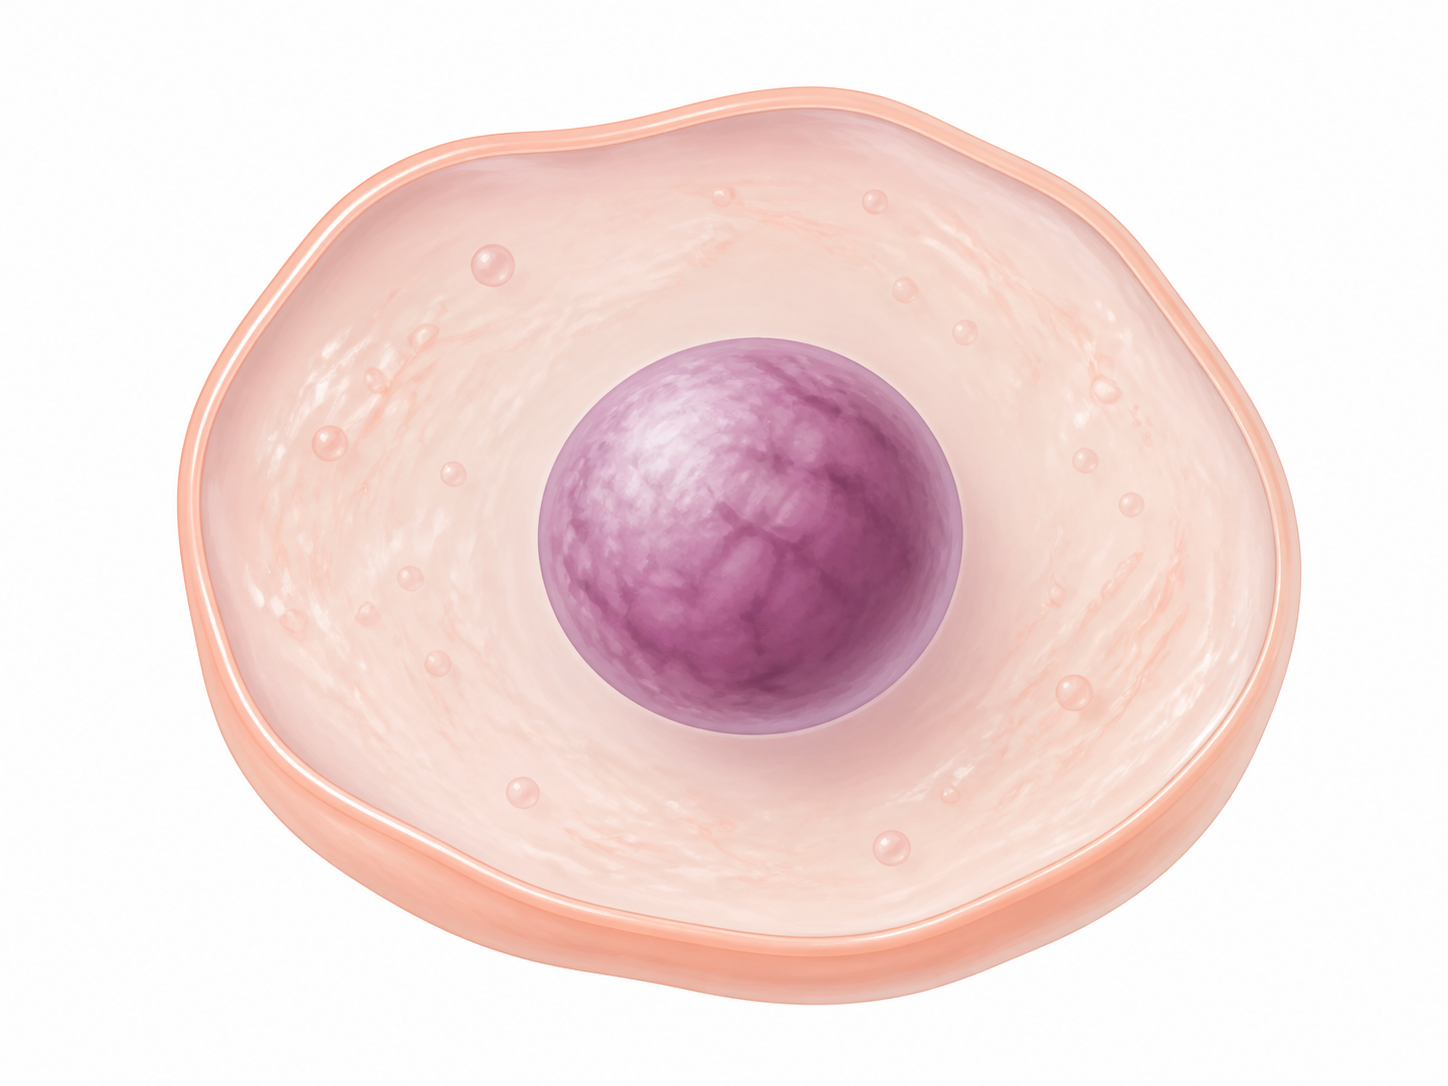
\includegraphics[width=0.9\linewidth]{images/book1/ai/fig-animal-cell.png}};
  \begin{scope}[x={(img.south east)}, y={(img.north west)},
      every node/.style={font=\footnotesize}]
    \draw[omDef, thick] (0.24,0.79) -- (0.12,0.93) node[above] {غشاء};
    \draw[omDef, thick] (0.32,0.42) -- (0.15,0.20)
      node[below] {سيتوبلازم};
    \draw[omDef, thick] (0.58,0.52) -- (0.80,0.20)
      node[below] {نواة};
  \end{scope}
\end{tikzpicture}

{\small \omterm{def:g5:first-look-at-cells:cell}{خلية} حيوانية:\\ \omterm{def:g6:cell-unit-of-life:parts}{غشاء}، \omterm{def:g6:cell-unit-of-life:parts}{وسيتوبلازم}، \omterm{def:g6:cell-unit-of-life:parts}{ونواة}}
\end{minipage}\hfill
\begin{minipage}[t]{0.48\linewidth}\centering
\begin{tikzpicture}
  \node[anchor=south west, inner sep=0] (img) at (0,0)
    {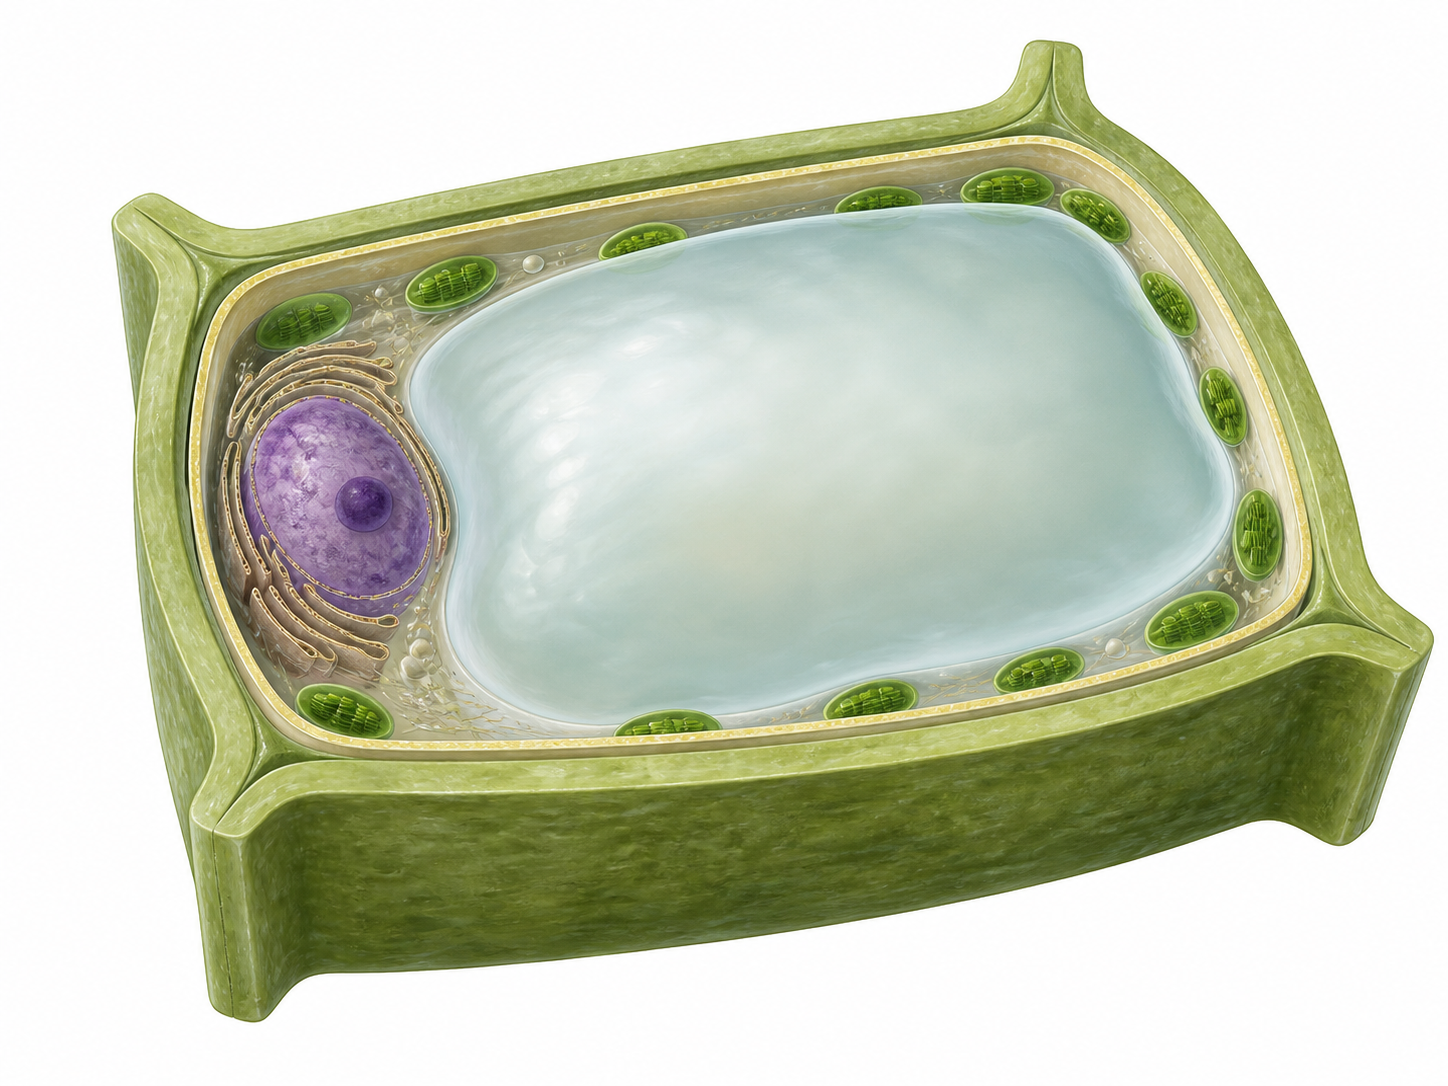
\includegraphics[width=0.98\linewidth]{images/book1/ai/fig-plant-cell.png}};
  \begin{scope}[x={(img.south east)}, y={(img.north west)},
      every node/.style={font=\footnotesize}]
    \draw[omMeth!60!black, thick] (0.16,0.80) -- (0.08,0.94)
      node[above] {جدار خلوي};
    \draw[omDef, thick] (0.26,0.53) -- (0.22,-0.04)
      node[below] {نواة};
    \draw[omMeth!60!black, thick] (0.72,0.24) -- (0.85,-0.04)
      node[below] {حبيبات خضراء};
    \draw[omDef!70, thick] (0.62,0.55) -- (0.70,1.04)
      node[above] {جيب ماء};
  \end{scope}
\end{tikzpicture}

{\small \omterm{def:g5:first-look-at-cells:cell}{خلية} نباتية: العدّة نفسها، مع جدار\\ وحبيبات خضراء وجيب
ماء}
\end{minipage}

\medskip
{\small الخليتان الكلاسيكيتان جنبًا إلى جنب. العدّة الثلاثية نفسها؛
\omterm{def:g5:first-look-at-cells:cell}{والخلية} النباتية تضيف جدارها وحبيباتها الخضراء وجيب مائها
الممتلئ.}
\end{omfigure}

\begin{example}[التمييز بين الشريحتين]\label{ex:g6:cell-unit-of-life:slides}
عند العودة إلى \omterm{def:g5:first-look-at-cells:microscope}{المجهر} بشريحتَي
\cref{ex:g5:first-look-at-cells:classics}، صارت للفروق أسماء.
قشرة \omterm{ex:g4:plants-without-seeds:bulbtuber}{البصلة}: جدران مستقيمة تلتقي عند زوايا --- وهي الجدران
الخلوية؛ \omterm{def:g6:cell-unit-of-life:parts}{ونواة} مدفوعة إلى الجانب --- من فعل جيب الماء. \omterm{def:g5:first-look-at-cells:cell}{وخلايا}
الخدّ: لا جدران، وحدود طرية مستديرة --- \omterm{def:g6:cell-unit-of-life:parts}{غشاء} فحسب --- \omterm{def:g6:cell-unit-of-life:parts}{ونواة} قرب
الوسط. فنظرة واحدة تقرأ الآن: نباتية أم حيوانية.
\end{example}

\section{حيوات كاملة في خلية واحدة}

\begin{definition}[الكائنات وحيدة الخلية]\label{def:g6:cell-unit-of-life:unicellular}
\omterm{def:g1:living-or-not:living}{الكائن الحي} \emph{وحيد الخلية}\index{وحيد الخلية} كائن كامل من
\omterm{def:g5:first-look-at-cells:cell}{خلية} واحدة بالضبط
(\cref{rem:g5:first-look-at-cells:onecelled}). ففي \omterm{def:g6:cell-unit-of-life:parts}{غشاء} واحد
يتغذى ويتحرك ويحسّ ويتكاثر --- بالانقسام إلى اثنين
(وهو انقسام \cref{prop:g5:first-look-at-cells:growth}، بوصفه حكاية
حياة كاملة). وخميرة \cref{ex:g6:producing-our-food:bread} واحدة
منها؛ وكذلك سابحات أي قطرة بركة، وأكثر \omterm{def:g6:producing-our-food:fermentation}{ميكروبات} \omterm{def:g6:decomposers-and-soil:soil}{التربة} واللبن
والأيدي.
\end{definition}

\begin{example}[جولة في قطرة ماء بركة]\label{ex:g6:cell-unit-of-life:drop}
قطرة واحدة من جدار الحوض الأخضر، تحت العدسة: \omterm{def:g5:first-look-at-cells:cell}{خلية} على شكل نعل
تجدّف مارّةً بأهداب تخفق، أسرع من كل ما في المرأى؛ \omterm{def:g5:first-look-at-cells:cell}{وخلايا} مفردة
خضراء --- منتِجات سابحة، تلتقط \omterm{def:g6:exploring-our-environment:conditions}{الضوء} كأي \omterm{def:g1:plants-around-us:parts}{ورقة}؛ وكتلة تسيل حول
غذائها فتبتلعه كله. كل واحدة تتغذى وتتحرك وتتجنب --- حياة \omterm{def:g1:animals-around-us:animal}{حيوان} أو
\omterm{def:g1:plants-around-us:plant}{نبات} كاملة، مُوازَنة في \omterm{def:g5:first-look-at-cells:cell}{خلية} واحدة.
\end{example}

\begin{remark}[خلية واحدة أو كثيرة: طريقتان للحياة]\label{rem:g6:cell-unit-of-life:twoways}
الكائن \omterm{def:g6:cell-unit-of-life:unicellular}{وحيد الخلية} يفعل كل شيء \omterm{def:g5:first-look-at-cells:cell}{بخلية} واحدة؛ وجسمك يفعل كل شيء
بعشرات آلاف المليارات منها، \emph{متخصصةً} --- \omterm{def:g5:first-look-at-cells:cell}{خلايا} خدّ للتبطين،
\omterm{def:g5:first-look-at-cells:cell}{وخلايا} عضلية \omterm{def:g3:bones-and-muscles:muscle}{تنقبض} (\cref{def:g3:bones-and-muscles:muscle})،
\omterm{def:g5:first-look-at-cells:cell}{وخلايا} عصبية تحمل رسائل
\cref{prop:g5:brain-in-command:loop}. \omterm{def:g5:first-look-at-cells:cell}{فالخلايا} الكثيرة تتيح تقسيم
العمل؛ \omterm{def:g5:first-look-at-cells:cell}{والخلية} الواحدة تعني كل صنعة في غرفة واحدة. وكلتا الخطتين
تنجح: فوحيدات \omterm{def:g5:first-look-at-cells:cell}{الخلية} أكثر \omterm{def:g6:exploring-our-environment:components}{الكائنات الحية} عددًا على الأرض.
\end{remark}

\section{النظرية الخلوية}

\begin{proposition}[النظرية الخلوية]\label{prop:g6:cell-unit-of-life:theory}
جملتان، استغرقتا قرونًا، تلخصان هذا الفصل
و\cref{ch:g5:first-look-at-cells}:
\begin{enumerate}
  \item كل \omterm{def:g6:exploring-our-environment:components}{كائن حي} مصنوع من \omterm{def:g5:first-look-at-cells:cell}{خلية} واحدة أو أكثر، وهي أصغر وحدات
        الحياة؛
  \item وكل \omterm{def:g5:first-look-at-cells:cell}{خلية} تأتي من انقسام \omterm{def:g5:first-look-at-cells:cell}{خلية} موجودة من قبل.
\end{enumerate}
ولم يُعثر على استثناء قط --- لا في أعمق بحر، ولا في أقدم غدير
صخري. وللجملة الثانية نتيجة جارفة: فكل \omterm{def:g5:first-look-at-cells:cell}{خلية} حية اليوم تواصل سلسلة
انقسامات لا انقطاع فيها ترجع إلى أوائل الحياة --- وهي \omterm{prop:g6:classification-kinship:kinship}{القرابة}
(\cref{prop:g6:classification-kinship:kinship}) مكتوبةً على مقياس
\omterm{def:g5:first-look-at-cells:cell}{الخلية}.
\end{proposition}
\admitted

\begin{method}[قراءة أي كائن على مقياس الخلية]\label{met:g6:cell-unit-of-life:read}
إذا واجهت أي \omterm{def:g6:exploring-our-environment:components}{كائن حي}:
\begin{enumerate}
  \item فاسأل أولًا: أخلية واحدة أم كثيرة؟
  \item فإن كانت كثيرة، فتوقّع أصنافًا متخصصة --- للتبطين،
        وللنقل، وللانقباض، وللقيادة؛
  \item وأنباتي هو أم حيواني؟ راجع الجدران والحبيبات الخضراء عند
        \omterm{def:g5:first-look-at-cells:microscope}{المجهر}؛
  \item وكل نمو أو إصلاح أو تكاثر ترصده: ترجمه إلى انقسامات
        \omterm{def:g5:first-look-at-cells:cell}{خلايا} --- فالجملة الثانية تضمن أن الترجمة موجودة.
\end{enumerate}
\end{method}

\begin{example}[النظرية في العمل في هذا الكتاب]\label{ex:g6:cell-unit-of-life:atwork}
الجملة الأولى سندت \omterm{prop:g5:first-look-at-cells:principle}{وحدة الحياة}
(\cref{prop:g5:first-look-at-cells:principle})؛ والجملة الثانية
سندت النمو بالانقسام
(\cref{ex:g5:first-look-at-cells:one})، وتضاعف \omterm{ex:g6:producing-our-food:bread}{الخميرة} في العجين،
وتكاثر المحلِّلين في الكومة الدافئة، وقوى \omterm{def:g6:producing-our-food:fermentation}{الميكروبات} العاملة في
\cref{ch:g6:producing-our-food}. نظرية صغيرة واحدة، تحمل حصة كبيرة
من أحياء هذه السنة.
\end{example}

\section{تمارين}

\begin{exercise}[$\star$]\label{exo:g6:cell-unit-of-life:1}
سمِّ عدّة الأجزاء الثلاثة في كل \omterm{def:g5:first-look-at-cells:cell}{خلية}، مع عمل كل جزء.
\end{exercise}

\begin{exercise}[$\star$]\label{exo:g6:cell-unit-of-life:2}
سمِّ زيادات \omterm{def:g5:first-look-at-cells:cell}{الخلية} النباتية الثلاث وما يفعله كل واحدة.
\end{exercise}

\begin{exercise}[$\star$]\label{exo:g6:cell-unit-of-life:3}
عند \omterm{def:g5:first-look-at-cells:microscope}{المجهر}، كيف تميّز \omterm{def:g5:first-look-at-cells:cell}{خلية} قشرة \omterm{ex:g4:plants-without-seeds:bulbtuber}{بصلة} من \omterm{def:g5:first-look-at-cells:cell}{خلية} خدّ؟ فرقان مرئيان.
\end{exercise}

\begin{exercise}[$\star$]\label{exo:g6:cell-unit-of-life:4}
ما \omterm{def:g1:living-or-not:living}{الكائن الحي} \omterm{def:g6:cell-unit-of-life:unicellular}{وحيد الخلية}؟ سمِّ اثنين من هذا الفصل.
\end{exercise}

\begin{exercise}[$\star$]\label{exo:g6:cell-unit-of-life:5}
اذكر جملتَي النظرية الخلوية.
\end{exercise}

\begin{exercise}[$\star$]\label{exo:g6:cell-unit-of-life:6}
كيف يتكاثر الكائن \omterm{def:g6:cell-unit-of-life:unicellular}{وحيد الخلية}؟
\end{exercise}

\begin{exercise}[$\star\star$]\label{exo:g6:cell-unit-of-life:7}
لماذا تقف \omterm{def:g1:plants-around-us:plant}{النباتات} بلا \omterm{def:g3:bones-and-muscles:skeleton}{عظام}؟ وأي قطعتين من عتاد \omterm{def:g5:first-look-at-cells:cell}{الخلية} النباتية
تتقاسمان العمل --- وما الذبول على مقياس \omterm{def:g5:first-look-at-cells:cell}{الخلية}؟
\end{exercise}

\begin{exercise}[$\star\star$]\label{exo:g6:cell-unit-of-life:8}
أي جزء من \omterm{def:g5:first-look-at-cells:cell}{الخلية} هو مشغل \omterm{def:g5:food-webs:roles}{المنتِجين} في
\cref{prop:g6:plants-are-producers:produce}؟ ولماذا يجب أن تفتقده
كل \omterm{def:g5:first-look-at-cells:cell}{خلية} حيوانية، وفق
\cref{prop:g6:matter-from-food:transform}؟
\end{exercise}

\begin{exercise}[$\star\star$]\label{exo:g6:cell-unit-of-life:9}
أعطِ ثلاثة أصناف من \omterm{def:g5:first-look-at-cells:cell}{خلايا} جسمك المتخصصة وصنعة كل واحد، من
\cref{rem:g6:cell-unit-of-life:twoways}.
\end{exercise}

\begin{exercise}[$\star\star$]\label{exo:g6:cell-unit-of-life:10}
ترجم إلى انقسامات \omterm{def:g5:first-look-at-cells:cell}{خلايا}، وفق
\cref{met:g6:cell-unit-of-life:read}: سحجة تلتئم؛ وعجين يتضاعف في
ليلة؛ وشرغوف ينمو.
\end{exercise}

\begin{exercise}[$\star\star$]\label{exo:g6:cell-unit-of-life:11}
سابحات قطرة البركة الخضراء \omterm{def:g5:first-look-at-cells:cell}{خلايا} مفردة تلتقط \omterm{def:g6:exploring-our-environment:conditions}{الضوء}. فأي صنعة من
صنعات \cref{def:g5:food-webs:roles} تجري عليها، وماذا يجعلها ذلك
في \omterm{def:g5:food-webs:web}{الشبكة الغذائية} للبركة؟
\end{exercise}

\begin{exercise}[$\star\star\star$]\label{exo:g6:cell-unit-of-life:12}
خذ الجملة الثانية من النظرية الخلوية مأخذ الجدّ، كما أخذت
\cref{rem:g6:classification-kinship:implies} الشجرة: أي سلسلة لا
انقطاع فيها تصل \omterm{def:g5:first-look-at-cells:cell}{خلية} من \omterm{def:g5:first-look-at-cells:cell}{خلايا} خدّك بالماضي البعيد؟ اذكر النتيجة في
جملة واحدة.
\end{exercise}

\section{مسألة: أصيل المجهر}

\begin{problem}[{مسألة نهاية الأسبوع --- أربع شرائح ونظرية
واحدة}]\label{pb:g6:cell-unit-of-life:1}
أصيل \omterm{def:g5:first-look-at-cells:microscope}{المجهر} عند الصف: أربع محطات وأربع شرائح --- قشرة \omterm{ex:g4:plants-without-seeds:bulbtuber}{بصلة} (أ)،
وكشط خدّ (ب)، وقطرة ماء بركة (ج)، ومسحة لبن (د). ويطوف كل فريق
المحطات الأربع ويحتفظ برسومه.

\medskip\noindent\textbf{القسم الأول --- المحطتان أ وب.}
\begin{enumerate}
  \item في المحطة أ يرسم الفريق ``طوبًا'' مستقيم الجدران، في كل
        واحدة بقعة داكنة منزوية إلى جانب. سمِّ الجدار، والبقعة،
        والمتّهم بالزحام.
  \item وفي المحطة ب: \omterm{def:g5:first-look-at-cells:cell}{خلايا} مستديرة، بلا جدران، وبقعها في الوسط.
        عدّد العتاد الذي في \omterm{def:g5:first-look-at-cells:cell}{خلايا} أ ويفتقده ما في ب --- والعدّة
        التي يشتركان فيها.
  \item يسأل زميل لماذا لا تُظهر \omterm{def:g5:first-look-at-cells:cell}{خلايا} \omterm{ex:g4:plants-without-seeds:bulbtuber}{البصلة}، وهي من \omterm{ex:g4:plants-without-seeds:bulbtuber}{بصلة} نمت
        تحت الأرض، حبيبات خضراء. أجب بعمل الحبيبات وعنوان \omterm{ex:g4:plants-without-seeds:bulbtuber}{البصلة}.
  \item \omterm{def:g5:first-look-at-cells:cell}{خلايا} مَن على الشريحة ب؟ اذكر ما يلزم من ذلك وفق الجملة
        الثانية من النظرية الخلوية: من أين جاءت كل \omterm{def:g5:first-look-at-cells:cell}{خلية} منها؟
\end{enumerate}

\medskip\noindent\textbf{القسم الثاني --- المحطتان ج ود.}
\begin{enumerate}[resume]
  \item المحطة ج: المجدّفة على شكل النعل، والسابحات الخضراء،
        والكتلة السائلة. سمِّ لكل واحدة أنشطة الحياة المرئية في
        دقيقة من المراقبة --- واستنتج ما كل واحدة.
  \item السابحات الخضراء \omterm{def:g5:first-look-at-cells:cell}{خلايا} مفردة ومع ذلك منتِجات. فأي قطعة من
        العتاد يجب أن يُظهرها الرسم لإثبات ذلك؟
  \item مسحة اللبن في المحطة د تُظهر \omterm{def:g5:first-look-at-cells:cell}{خلايا} صغيرة جدًّا مزدوجة
        ومتسلسلة بأعداد هائلة. اربطها بما في
        \cref{ex:g6:producing-our-food:yogurt}: ماذا فعلت هذه
        \omterm{def:g5:first-look-at-cells:cell}{الخلايا} \omterm{def:g2:animals-grow-up:born}{بالحليب}، وما هي بمعجم هذا الفصل؟
  \item يزعم فريق أن الشريحة د لا تُظهر ``كائنات حية بل مجرد
        ذرّات''. فأي رصد واحد --- مع الصبر أو شريحة دافئة ---
        يحسم أتحيا الذرّات أم لا، وفق الجملة الثانية من النظرية
        الخلوية؟
\end{enumerate}

\medskip\noindent\textbf{القسم الثالث --- كتابة التقرير.}
\begin{enumerate}[resume]
  \item على التقرير أن يفرز الشرائح الأربع بحسب: أخلية واحدة أم
        كثيرة؟ أنباتية أم حيوانية أم لا هذه ولا تلك؟ افعل ذلك.
  \item كل رسم من رسوم الأصيل يُظهر عدّة الأجزاء الثلاثة نفسها.
        اذكر العدّة، وعلام يدل عمومها
        (\cref{prop:g5:first-look-at-cells:principle}).
  \item يختم المعلم: ``كل ما رسمتموه اليوم كان يومًا \omterm{def:g5:first-look-at-cells:cell}{خلية}
        واحدة.'' دافع عن الجملة في \omterm{ex:g4:plants-without-seeds:bulbtuber}{البصلة}، وفي صاحب \omterm{def:g5:first-look-at-cells:cell}{خلايا} الخدّ،
        وفي سلاسل اللبن.
  \item صُغ ما وجدتموه في الأصيل نظريةً خلوية --- جملتين ---
        وعلّم لكل شريحة أي جملة مثّلتها أحسن تمثيل.
\end{enumerate}
\end{problem}
